%!TEX TS-program = pdflatex
%!TEX root = i3det-top.tex
%!TEX encoding = UTF-8 Unicode

% additional definitions
\newcommand{\degC}[1]{$\unit[#1]{^\circ{C}}$}
%\newcommand{\mA}{\mbox{\unit{mA}}}
% definition to produce a "less than or similar to" symbol
\def\lsim{\mathrel{\rlap{\raise 0.2ex\hbox{$\,<\,$}}{\lower 0.9ex\hbox{$\,\sim\,$}}}}
% definition to produce a "greater than or similar to" symbol
\def\gsim{\mathrel{\rlap{\raise 0.2ex\hbox{$\,>\,$}}{\lower 0.9ex\hbox{$\,\sim\,$}}}}


\section{The Digital Optical Module}
\textsl{(Chris Wendt; 10 pages)}

\subsection{\label{sec:dom_functional} A Functional Description of the DOM}

The DOM (Figure~\ref{fig:domcomponents}) is the fundamental data acquisition
unit for IceCube, 
containing a downward-facing $10^{\prime\prime}$ diameter photomultiplier tube (PMT)
and associated circuit boards that allow near-autonomous operation.
Data acquisition, control, calibration, communication and low voltage power conversion 
are integrated in one annular circuit board that fits around the neck of the PMT (Main Board, Section~\ref{sec:mb})~\cite{ref:domdaq}. 
Separate circuit boards generate PMT high voltage, interface to the PMT pins~\cite{ref:pmt},
delay PMT signals, and generate calibration light flashes that can reach other DOMs.
Key requirements for the DOM include
the precise recording of a wide variety of PMT pulse widths and amplitudes, robustness in
a challenging deployment environment, and long term reliability.

The PMT detects
signals from neutrino events ranging over energies \unit[10]GeV--\unit[10]PeV
and  distances  from a few meters to \unit[500]m away.
Corresponding PMT waveforms can have amplitudes from \unit[1]mV up to and beyond the linearity limit
of the PMT (\unit[$\sim2$]volts) and widths from \unit[12]nsec to \unit[1500]nsec.
In order to accommodate such a variety of signals,
the DOM includes multiple digitizers with overlapping dynamic range and different sampling speeds
~\cite{ref:domdaq}.
Each DOM is triggered independently by detection of individual photons, starting a 
recording of the PMT waveform that includes further photons arriving up to \unit[6.4]{$\mu$sec} later.
The trigger time is saved along with the
waveform shape, which reveals the times of arriving photons relative to this reference.
The DOM typically accumulates such triggered data for a period of ? to \unit[?]sec before sending as a block.

DOMs transmit their data to computers in the IceCube Laboratory building using a twisted wire pair that also provides
power.  Wire pairs are bundled together to form the vertical down-hole cables and the horizontal surface cables.  
Each wire pair is shared between two DOMs, with data transfers initiated by a surface computer.
Separately, dedicated wiring to neighbor DOMs above and below allows 
quick recognition of local coincidences where nearest or next-to-nearest neighbors trigger within
a common \unit[1]$\mu$sec time window.
Local coincidence triggers often have complex PMT waveforms reflecting multiple photons
detected in each DOM, which are therefore
saved in full detail; otherwise the DOM saves abbreviated information appropriate to single photon
detection ~\cite{ref:domdaq}.

The DOM is capable of interpreting commands from the surface that specify tasks for configuration, 
data taking and transmission, monitoring or self-calibration.
Self-calibration functions establish PMT and amplifier gains as well as sampling speed.
The RAPCal system~\cite{ref:domdaq} is implemented for tracking each local DOM clock's offset from universal time,
allowing PMT pulses that were independently recorded in many DOMs  to be recombined into events by surface computers.

\subsection{\label{sec:dom_components} Components}

\subsubsection{\label{sec:sphere}Glass Sphere and Harness}

The glass sphere housing has diameter $13^{\prime\prime}$ and thickness $0.5^{\prime\prime}$.  
Spheres are specified to protect the inside electronics and PMT against long term applied pressure of 
\unit[250]bar (\unit[2.6]km water depth)
as well as temporary overpressure up to \unit[690]bar during refreezing of melted ice in the drill hole.
They were produced by Benthos, Inc., based on a design for deep sea environments but using glass
with very low potassium or other radioactive trace elements that would contribute to the dark noise
count rate (Section~\ref{sec:darknoise}).  
%N.B. not borosilicate, according to analysis shown at final CDR 2005 (Claire's slides), in contrast
%to the Benthos sphere datasheet which says borosilicate
Optical transmission was measured for representative samples as 93\% at \unit[400]nm,
decreasing to 50\% at \unit[340]nm and 10\% at \unit[315]nm (normal incidence, excluding Fresnel reflection).

Each sphere is assembled from two hemispheres that
mate precisely at the equator; after evacuating and backfilling with dry nitrogen, a butyl rubber
sealant is applied around the seam, and covered with wide plastic tape.
The interior gas pressure is set to 0.5 bar so the seal remains tight even
at ambient south pole air pressure 0.6 bar.

The DOM is held by an aluminum band with rubber gaskets against
the glass above and below the equator seam. 
Figure~\ref{fig:domharness} shows how it is attached to the main down-hole cable via a system
of steel rope and chain that carries the weight load around the DOM.
The main cable bends around the DOM, and the DOM axis stays vertically aligned with the string.


%NK section 3.4.1 text:
%The spherical pressure housing consists of two hemespheres made of low expansion borosilicate
%glass that seal at the equator. Each pair of mating hemespheres have been tested for pressure
%tightness at 10,000 psi (689 bar) by the manufacturer. [The pressure must operate continuously
%under 250 bar (2.6 km-deep water) and allow the over pressure of 689 bar (refreezing pressure) for
%seven days. 9400-0029-PCR.] The top hemesphere has a 16.3 mm-diameter hole for installing the
%penetrator assembly (below) that facilitates electrical connections to the interior electronics without
%compromising the pressure tightness.
%The pair of glass hemespheres consitutes more than 9 Kg of mass (9.07 Kg) and is potentially a
%significant source of photonic noise arising from the decay of radioisotope content. The IceCube
%spheres are produced with a special attention to eliminate pottasium content and minimize other
%radioactive trace elements, such as cerium. [According to Chemir Analytical Services report, June
%2005, the pottasium concentration was below the detection level and that of cerium was less than
%40 ppm by ICP analysis; however, in a separate University of Washington measurement, non-zero
%numbers are seen under pottasium. Without any write up to accompany the measurement, we
%don’t know how to interpret the numbers.] The manufacturer’s standard material contains CaCO3
%(calcite), known to have fluorescent properties, which was also eliminated [Presumably. See Kael’s
%report, November 2003]. 

\subsubsection{\label{sec:penetrator}Cable Penetrator, Cable and Connector}

%NK section 3.4.2 text:
%(This includes the external umbilical, the internal pigtail, and the connectors on either end.) Each
%DOM requires three wire-pair connections to its interior: one pair is connected to the surface DAQ
%system and carries the bidirectional communication signals and power; another two pairs provide
%local coincidence connections to the neighboring DOMs, one above and one below.
%The penetrator is an assembly of cables and electrical feedthrough that accomplishes the 
%necessary electrical connections from outside the pressure housing through its wall while maintaining the
%pressure-tightness, characteristic impedance, and signal cross-talk requirements. It consists of a
%threaded stainless steel feedthrough that achieves the pressure-tightness by means of a single
%o-ring pressed against the glass exterior and is tightened with a spring washer and a locking nut
%from inside; a pig-tail cable that connects to the DOM main board; and a custom-designed umbili-
%cal cable containing three shielded twisted-pair cables within its jacket and having a pressure-tight
%multi-pin connector that plugs into the mating connector at one of the breakouts (see below) of the
%main cable. The umbilical cable is 0.7 m long for the type U DOM and 19.2 m long for the type T
%DOM. The umbilical cable is terminated with a dissimilar connector depending on the type of the
%DOM in order to avoid a wrong connection by human error during the deployment.

A customized penetrator assembly brings three wire pairs out through a \unit[16.3]mm hole in
the DOM glass.  They are routed inside the umbilical cable, visible in Figure~\ref{fig:domharness},
and terminate at a pressure-tight, waterproof connector that mates with a similar connector
and thus continues each pair into the main cable.  One wire pair connects ultimately with a 
computer in the IceCube Laboratory building, carrying power and the bidirectional digital
communications stream.  
%The figure referenced is like NK Figure 3 "In-ice DOM connections"
The other two pairs lead to neighbor DOMs directly above and below (Figure~\ref{fig:lc}),
carrying local coincidence digital pulses that signify time correlated hits in nearby DOMs (Section~\ref{sec:mb}).

The penetrator itself is a customized stainless steel feedthrough, with a plastic shell that is also molded onto
the umbilical cable jacket.  
The penetrator has an o-ring seal facing the glass outside and is secured by a nut inside the sphere.  
External mechanical features like the penetrator are subject to large stresses during deployment and the refreezing process;
the right angle bend was chosen for robustness, based on previous experience deploying AMANDA modules.
The complete assembly, including umbilical cable and type XSJJ connector, was produced by SEACON (California).  


\subsubsection{\label{sec:pmt}PMT, Gel and Magnetic Shield}

%NK text: The gel’s primary purpose is optical coupling between the sphere and the PMT; 
%however, it also serves as a mechanical shock absorber to protect
%the PMT and the electronic assemblies during the handling, transport, and deployment. All other
%components are mounted on the PMT and no components make a mechanical contact with the
%pressure housing wall, except for the pigtail cable of the penetrator.

DOMs use the $10^{\prime\prime}$ diameter Hamamatsu R7081-02 PMT, 
or the corresponding high-quantum-efficiency (HQE) version for Deep Core strings.
Its properties have been measured and described in \cite{ref:pmt}.  It is specified by Hamamatsu for
the wavelength range \unit[300]nm--\unit[650]nm, with peak quantum efficiency around 25\% (34\% for HQE)
near \unit[390]nm.  It features a box-and-line dynode chain with 10 stages, and is operated at gain $10^7$
(Section~\ref{sec:domcal}).

The PMT bulb faces downwards in the bottom glass hemisphere, secured in high-strength 
silicone gel to a depth surrounding the photocathode area.  
The gel provides mechanical support for the whole assembly of PMT and circuit boards,
as well as good optical coupling.  
Gel thickness between PMT envelope and glass sphere is approximately \unit[1]cm.  
Originally the gel was supplied as General Electric RTV6136-D1,
and later as a similar formulation from Quantum Silicones (Virginia, USA).  
It is optically clear with transmission 97\% at \unit[400]nm, 91\% at \unit[340]nm, and 65\% at \unit[300]nm
(normal incidence).  The refractive index is 1.41, yielding less than 0.1\% Fresnel reflection as light
passes from the sphere glass into the gel and then into the PMT envelope.
The characteristics of the cured gel are specified to remain stable in the temperature range $-70^\circ$C to $45^\circ$C.

To reduce effects of the ambient magnetic field (\unit[550]mG, $17^\circ$ from vertical), a mu-metal cage surrounds the PMT bulb up to
the neck join.  It was constructed as a wire mesh with typical wire spacing \unit[66]mm and
wire diameter \unit[1]mm, blocking about 4\% of the incident light.
The resulting interior magnetic field is a factor 2.8 below
the external field, pointing mostly along the axis and therefore reducing efficiency by
less than 2\% for this type of PMT~\cite{ref:calvo}.

Other interior DOM components are held in place by attachment to the PMT, mostly via screws into
a molded plastic collar glued around the neck.  The PMT base board is soldered directly to the pins.


\subsubsection{\label{sec:mainboard}Main Board and Delay Board}
The Main Board and its operation has been described in detail in \cite{ref:domdaq}.  
It interfaces to other boards as shown in
%figure here is NK Figure 4 "Functional Block Diagram of the DOM"
Figure~\ref{fig:domelectronics} and itself provides many key functions of the DOM:

%text from NK section 3.5.1
\begin{itemize}
\item{Control all the devices inside the DOM, including the high voltage power supply for the PMT, 
the flasher board, and various sensors (pressure, temperature, power supply voltage monitor). 
Also supply necessary DC power to the subsystems.}
\item{Digitize the PMT waveforms, using the custom ASIC (ATWD: analog transient waveform digitizer) and a continuous sampling ADC.}
\item{Carry out computing functions. This includes executing PMT gain calibration, compressing 
the digitized waveform, temporarily storing the data, creating data packets and time stamping them.}
\item{Communicate with the data acquisition system on the surface.}
\item{Exchange timing pulses with the surface DAQ to calibrate the internal DOM clock. }
\item{Exchange ”local coincidence” pulses with the adjacent DOMs.}
\end{itemize}

PMT waveforms are captured by the ATWD chips with sampling period \unit[3.3]nsec, starting after 
a discriminator trigger is recognized by the sequencing logic.  The total sampling interval is \unit[427]nsec,  
encompassing the time spread of most photons arriving from up to \unit[100]m away.
The Delay Board is connected between
the discriminator and the ATWD preamplifiers, adding a pretrigger window in this recorded waveform
that allows precise fitting of the leading edge time.  It contains a \unit[$\sim10$]m long, \unit[0.25]mm
wide, serpentine copper trace embedded in the dielectric and sandwiched between ground planes,
giving a total delay of about \unit[75]nsec.  After accounting for triggering delays, this causes the
waveform recording to start at least \unit[10]nsec before the leading edge time.
 
%NK section 3.5.2 text:
%Although low-power and high-speed, the ATWDs must be initiated by a trigger signal in order to start
%the digitizing operation. In order to capture the front pedestal of the waveform, the PMT signal is
%split in two ways: one branch enters the trigger circuit and initiates the ATWD and the other branch
%enters the delay line and emerges in the analog input of the digitizer after ?75 ns. The delay line
%is a stripline implemented as a ?10 m-long, 0.25 mm-wide, serpentine copper trace embedded in
%the dielectric and sandwiched between ground planes of the delay board. Unlike a coaxial cable
%delay line, the delay board is compact and easy to integrate into the limited space in the DOM
%sphere: the board is 3.2 mm thick and has the same area profile as the main board, below which
%it is mounted.
%(The impedance is 95 Ω. The delay time is 75±2 ns. The risetime and falltime is typically 3 ns
%(Including the source profile. ERD, Fig. 2). The signal attenuation is required to be less than 12\%.
%%The trace width was measured from ther gerber file. The trace length is based on the delay of
%0.166 ns per inch, found in the simulation file found on docushare, Document-6600.)

%%%%%%%%%%%%%%%%%%%%%%%%%%%%%%%%%%%%%%%%%%%%%%%%%%%%%%
%%[Below is more text that is too much detail for this paper]
%Several features are included for calibration functions of the DOM, also used for self-test.
%Each DOM has a local clock driven from a high-stability \unit[20]MHz(?) oscillator, in terms of which all local
%times are measured.  In order to determine slowly drifting offsets between clocks in each DOM and a master
%surface clock, the DOM provides waveform digitization of a regular timing pulse sent from the surface, as 
%well as sending a return pulse (Section~{sec:rapcal})~\cite{ref:domdaq}.
%For calibration of the waveform digitizers, the DOM has a pulser circuit that can inject programmed amounts of
%charge into the front end circuitry, and has an input multiplexer that allows the (adjustable) sampling rate
%to be calibrated via the clock oscillator.  
%A pulsed LED facilitates calibration of gain and time delay in the PMT as a function of applied high voltage 
%(Section~{sec:domcal}).

%During the first \unit[427]nsec recording interval, information is captured in one of two analog transient 
%waveform digitizers (ATWDs)
%with sampling period \unit[3.3]nsec, single bit resolution \unit[0.1?]mV for small signals and dynamic range
%\unit[7?]volts.  This period encompasses the time
%spread of most photons arriving from up to \unit[100]m away. 
%An analog delay line causes the recording to include a pretrigger period of at least \unit[10]nsec,
%allowing the leading edge to be measured with \unit[1]nsec resolution.
%For multi-photon pulses, the full arrival time profile can be reconstructed by fitting the waveform 
%as a sum of single photon responses, each contribution having typical amplitude
%\unit[5]mV and width \unit[12]nsec FWHM.
%The upper end of the dynamic range accommodates the full
%linear response range of the PMT, up to about 400(?) photoelectrons per \unit[15]nsec\cite{ref:pmtpaper}, 
%as well as fully saturated PMT pulses around \unit[5]volts amplitude.

%While the ATWDs are optimized for multi-photon events that are close to the DOM, the information
%content is more than needed for single isolated photon detections far away from the interaction,
%which may also be spread over a longer time period.
%Accordingly, the FADC is a separate 10-bit digitizer that records PMT waveforms for up to 
%\unit[6.4]{$\mu$sec} but with coarser sampling interval \unit[25]nsec.  
%This channel includes an anti-aliasing filter to broaden
%individual photon responses to \unit[70?]nsec FWHM and peak amplitude \unit[1]mV.
%With amplitude resolution \unit[0.1]mV, photon arrival times can still be determined to within \unit[7?]nsec.

%In order to quickly identify close-by events requiring full ATWD information, the cabling system includes
%extra wiring for DOMs to communicate directly with neighbors above and below~\cite{ref:domdaq}.  
%Each DOM trigger can 
%thus be quickly classified by whether a nearest or next-to-nearest neighbor DOM also
%triggered within a \unit[$\pm$1]$\mu$sec time window.  Such a local coincidence causes the full length
%ATWD and FADC waveforms to be saved, and otherwise only three FADC samples are saved along with
%the reference timestamp.
%%[End of text that is too much detail for this paper]
%%%%%%%%%%%%%%%%%%%%%%%%%%%%%%%%%%%%%%%%%%%%%%%%%%%%%%



\subsubsection{\label{sec:hv}HV Supply and Divider}

The PMT high voltage subsystem consists of a resistive voltage divider circuit (PMT Base) directly
solder-mounted on the PMT and a separate high voltage control board. 
The high voltage control board includes a DAC and an ADC for setting and reading out the PMT high voltage,
connected to the Main Board with a digital interface.  It also holds the high voltage generator, which
is a custom encapsulated module designed by EMCO (California).  The maximum high voltage is
\unit[2047]volts, specified for up to \unit[30]$\mu A$ current.  The set voltage is proportional to the DAC
output, and the actual voltage is monitored via a high-impedance divider and the ADC.  The output ripple
is less than \unit[1]mV, and stability is better than \unit[200]ppm over 8~hours.  Power consumption is
\unit[300?]mW at full load.

The generator output is carried to the PMT Base Board via a high voltage coaxial cable.  This board is
described in \cite{ref:pmt}.  Its voltage divider presents a total resistive load of \unit[130]M$\Omega$.
The PMT is operated with cathode at ground potential, so the anode signal output is AC coupled using 
a 1:1 bifilar wound toroid transformer mounted on the Base Board.
The transformer secondary is then wired to the Main Board analog input with a coaxial cable.

%NK section 3.5.3 text:
%The high-voltage subsystem consisits of a resistive voltage divider circuit (PMT base board) directly
%solder-mounted on the PMT and a separate high-voltage control board, consisting of a modular
%high-voltage generator and a digital interface to the main board, which provides a +5 V DC power,
%issues the on/off command, sets the high voltage output by controlling the DAC, and monitors the
%precisely scaled down value of the high voltage output by reading the ADC. The output of the
%high-voltage generator is delivered to the PMT base board by way of a high-voltage coaxial cable
%(a “pig tail” cable) originating from inside the high voltage generator. The high-voltage generator
%is modular in the sense that all the high voltage circuitry is encapsulated in this unit. Having no
%high voltage nodes exposed to anywhere other than the PMT base board allows all the failure
%mechanisms inherent to high voltage circuitry to be completely isolated within the high voltage
%generator module and the PMT base board.
%(a) PMT Base Board The design of the PMT base board in relation to the performance of the
%PMT has been already discussed in some detail in our earlier paper[3]. Here, we outline only the
%salient features. The PMT base board has been designed to minimize the power consumption while
%meeting all the performance requirements. The base board supports 1 kHz of coninuous noise
%pulses and large (explain) isolated transient pulses lasting as long as 1 us. The total resistance is
%130 MΩ, which corresponds to the maximum bleeder current of 15 ?A and the power dissipation
%of less than 30 mW. The divider ratios have been optimized for the optimum operation (maximum
%collection efficiency) of the PMT when operated at the nominal gain of 107; since the PMT has a
%manufacturing spread, this corresponds to the anode voltage of 1050 to 1600 V. Since the PMT
%operates with the cathode at ground potential (for unknown historical reasons), the PMT pulse
%signals are ac-coupled from the high anode potential to the analog front-end of the main board,
%where the digitization takes places. The ac-coupling is accomplished using a custom-designed
%1:1 bifilar-wound toroidal transformer mounted on the PMT base board. Transformer-coupling is
%reliable and virtually noise-free for our purposes unlike capacitive-coupling.
%For reliability, the circuit has been implemented using through-hole components as much as pos-
%sible, except for several low-voltage nodes where a smaller low-inductance components are pre-
%ferred. The circuit has been designed to ensure that no component is under more than 50% of the
%its rated voltage. In order to eliminate the possibility of a corona discharge, all the through-hole
%solder joints have been shaped as a smooth ”dome” by a specially-developed manufacturing tech-
%nique involving two passes of wave-soldering process (Maybe Pensar’s permission is needed to
%disclose this?).
%(b) High Voltage Generator and Control Board The high voltage generator receives a +5 V
%DC power from the main board and generates a high voltage of up to 2047 V. It has been custom-
%designed[6] for low-power, low-noise, and high reliability. The proprietary circuit consists of a quasi-
%sine oscillator running at a few 100 kHz, whose output is transformer-coupled to a diode rectifier
%circuit, low-pass filtered, and fed back to the oscillator. (This description is based on the block
%diagram of the CA Series product datasheet from EMCO website[7]. The IceCube high-votage
%generator is a customized version of this series of products.) The circuit is potted inside a steel
%case and the high voltage output exits the unit via a “pig tail” cable that reaches the PMT base
%board. The unit is compact (7 x 2.8 x 1.4 cm3) and weighs about 60 grams. The output voltage of
%the generator has a very low ripple on the order of 1 mV (spec’ed as less than 2.4 ppm, DC to 20
%MHz) and is very stable (spec: 200 ppm variations over 8 h; maybe there are actual data showing
%the stability?). The unit can source up to 30 ?A of continuous current and dissipates less than 300
%mW of power under a full power operation. The unit is capable of starting up from a cold soak
%(non-operating storage) at -55°C.

\subsubsection{\label{sec:flasher}Flasher Board}
%NK section 3.5.4 has extensive description and simplified diagram

Each IceCube DOM contains a flasher board. The standard IceCube
flasher board, which is included in every DOM except the color DOMs
described below, is a circular board fitted with 12 LEDs (ETG-5UV405-30) with a peak
wavelength of 399~nm; the FWHM of the LED spectrum is
14~nm. The LEDs are arranged in pairs, evenly spaced around the board
with a 60$^{\circ}$ separation between each pair. One LED in each pair
points outward horizontally, the other LED is tilted upward at an angle
of 48$^{\circ}$, which is close to the Cherenkov angle in ice (n =
1.36). The angular emission profile of each LED has a FWHM of
30$^{\circ}$ in air, which is modeled as a Gaussian emission profile
with $\sigma = 13^{\circ}$. After refraction through the DOM glass and into
the ice, the value of $\sigma$ is 9.7$^{\circ}$ in the polar direction
and 9.8$^{\circ}$ in the azimuthal direction for the tilted LEDs, and  9.2$^{\circ}$ in the polar direction
and 10.1$^{\circ}$ in the azimuthal direction for the horizontal LEDs.

The LEDs are controlled by a current pulse applied to each LED through
a high speed MOSFET driver with a series resistor. The LEDs can be turned on individually or in any
combination of the 12, using a bitmask in the flasher DAQ
configuration. The photon output of the LED depends on the width and
brightness, or
amplitude of
the driving current pulse. The current amplitude is controlled by the
brightness setting in the flasher DAQ, which may have a value between
0 and 127; the maximum LED
current is 240~mA. The current pulse width is controlled by the width
setting in the flasher DAQ, which is twice the current pulse width in
nanoseconds and may have a value between 0 and 127; the maximum current pulse width is 70~ns. The
minimum stable pulse width that we can achieve is about 6~ns. The
photon output is related to the brightness  and width by the following
empirically derived relationship:
\begin{equation}
N = 1.17 \times 10^{10} \left (0.0006753 + 0.00005593B \right ) \left
  (W + 13.9 - \frac{57.5}{1 + B/34.4} \right )
\end{equation}
where N is the number of photons, B is the brightness setting (maximum
value 127) and W is the width setting (maximum value 127). The photon
output per LED ranges from $10^6$ to $10^{10}$ photons per flash,
which is equivalent to the energy output of GeV - 100 TeV cascades. The maximum
LED pulse rate is 610~Hz. The current waveform is read out by ATWD
digitizer channel~3 during flasher operation in order to measure the
precise rise time of the flasher pulse. The flasher light output
begins 8.3~ns after the current pulse is recorded. Although flashers can be
operated in multiple DOMs in the same run, the DAQ does not support
time-synced flashing of LEDs on different DOMs, so coincident flasher
events happen only by chance. 

The flasher LEDs are used for a variety of calibration purposes:
\begin{itemize}
\item verifying the timing response of the DOMs throughout the
  software
\item measuring the position of the deployed DOMs in ice
\item measuring the optical properties of the ice
\item verifying the performance of cascade reconstruction algorithms
  in measuring position, direction and energy
\end{itemize}

{\it Color DOMs}

There are 16~DOMs (8 on string~79 in the center of IceCube, 8 on
string~14 on the edge of IceCube) fitted with multiwavelength flasher boards, called
color DOMs or cDOMs. Each cDOM includes 3 LEDs with a nominal
wavelength of 505~nm, 3 LEDs with a nominal wavelength of 450~nm, 3
LEDs with a nominal wavelength of 370~nm and 3 LEDs with a nominal
wavelength of 340~nm. The LEDs are arranged in pairs as on the
standard flasher board, but all LEDs point outward horizontally. The
arrangement of the pairs is shown in Figure XXcdom sketch from cdom
wikiXX. The properties of the LEDs are given in
Table~\ref{table:cdom_properties}.

\begin{table}
\caption{Properties of the cDOM LEDs}
\begin{tabular}{|c|c|c|c|c|c|c|}
  \hline
 LED& nominal $\lambda$ & measured $\lambda$ & $\sigma$ air & $\sigma$
 DOM, polar & $\sigma$ DOM, azimuthal \\
\hline
UVTOP335-FW-TO39 &340 nm&338 nm&	51.0$^{\circ}$ &	36.1$^{\circ}$ &	42.9$^{\circ}$\\
\hline
NS370L\_5RFS &370 nm&	371 nm&55.2$^{\circ}$&	39.1$^{\circ}$&	42.9$^{\circ}$\\
\hline
LED450-01 & 450 nm& 447 nm&	6.8$^{\circ}$ &	4.8$^{\circ}$ &	5.3$^{\circ}$ \\
\hline
B5-433-B505 & 505 nm& 494 nm& 6.4$^{\circ}$ &	4.5$^{\circ}$ 	&4.9$^{\circ}$ \\
\hline
\end{tabular}
\label{table:cdom_properties}
\end{table}

\subsection{\label{sec:dom_prodtest}  Production and Testing}

\subsection{\label{sec:dom_calibration}  Calibration}

\subsubsection{\label{sec:domcal} DOMCal}

The calibration of the PMT waveforms recorded by the DOMs, i.e. translation
of digitized samples into voltage and time, as well as the gain of the PMT
itself, is achieved via DOM-by-DOM calibration constants determined by the
modules themselves.  The calibration software, DOMCal, uses precision calibration
circuits on the DOM Main Board as well as single photons as inputs
for a ladder of calibration routines.  Analysis and fitting of the
calibration results is done by the DOMCal software, with the results being
transmitted from each DOM to the surface as an XML file of fit parameters.

%The ladder of calibration routines is shown in
%Fig.~\ref{fig:domcal_ladder}.
The primary reference inputs to the calibration are a precision electronic
pulser circuit providing known charges; a circuit providing a reference DC
bias voltage level; the 20 MHz oscillator on the Main
Board, used as the timing reference; and single photoelectrons, either from
ambient ``dark noise'' photons or a low-luminosity LED on the Main Board.

Because the operating conditions for
the in-ice DOMs are so stable, DOMCal is only run once a year on the full
detector. IceTop DOMs are calibrated once per month.  Calibration is
typically performed on half the detector at at time, the other half
remaining in data-taking mode.  Because the calibration procedure produces
light, however, these runs are not used in normal analysis.

% FIX ME: ATWD reference?

First, the discriminator circuits used to trigger the DOM are calibrated
using the electronic pulser circuit.  This calibration is later refined using actual
PMT waveforms, once the PMT gain is known.  Next, the ATWD voltage levels
are calibrated by sweeping the input DC bias voltage and recording the
response; because of the slight variations in the ATWD circuits, this
calibration is produced for every sample and every channel.

This ATWD calibration also in principle allows determination of the baseline
voltage levels of each channel, needed for charge integration.  However, in
practice, these baselines are extremely sensitive to the operation
condition of the DOMs, and since data-taking conditions cannot be exactly
replicated while running DOMCal, the baselines used during data-taking are
determined instead by using averaged forced triggers taken during a normal
run.  DOMCal can still use its own baselines, though, for charge integration
during the calibration procedure.

The highest-gain channels of the two ATWDs are calibrated using the electronic
pulser circuit, and then the gains of the other ATWD channels and the FADC
are determined by varying the pulser output and comparing the charges
simultaneously recorded in multiple gain channels.  This relative
calibration is later refined using PMT waveforms stimulated by the Main
Board LED.

The ATWD sampling speed is calibrated by digitizing the Main Board oscillator
waveform and recording the number of clock cycles as a function of ATWD
speed setting.  The FADC sampling speed is slaved to the 20 MHz
oscillator, which is used as a timing reference.  The relative timing of
the ATWD and FADC waveforms is determined using the electronic pulser circuit;
non-linear fitting of the digitized waveforms to known templates is
required in order to determine the FADC offset to the required accuracy.
The transit time of the PMT and delay board as a function of PMT high
voltage is determined by calculating the delay between the digitized
current pulse through the Main Board LED and the observed light pulse in
the ATWDs.   

The PMT gain as a function of high voltage is calibrated using ambient
``dark noise'' photons --- the charge $e$ prior to amplification is quantized
and known.  At each voltage level, a histogram of many waveform charges is recorded,
and each histogram is fit with an exponential plus Gaussian model (see
Fig.~\ref{fig:domcal_hvfit}).  The peak of the Gaussian component is used to
determine the amplification of the PMT at each voltage, and a linear fit
of $\log_{10}(\mathrm{gain})$ versus $\log_{10}(\mathrm{voltage})$ allows
the high voltage of each PMT to be tuned to desired operating point ($10^7$
for in-ice DOMs; see Fig.~\ref{fig:domcal_hv_settings}).  Small ($3-5\%$)
corrections to the gain of each DOM are determined using charge
distributions recorded during normal data-taking; this corrects for a small
systematic difference in the charge as determined by DOMCal's integration
and the waveform pulse unfolding used in data processing.

% From JK DOMCal Hist.ipynb
\begin{figure}[!h]
 \centering
 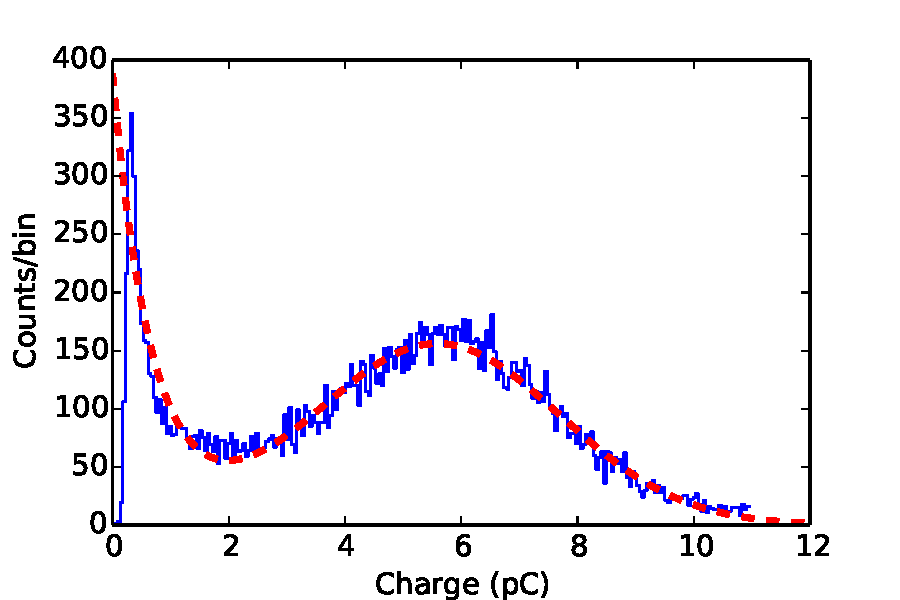
\includegraphics[width=0.6\textwidth]{graphics/dom/domcal/hvfit.pdf}
 \caption{Sample SPE charge spectrum as recorded by DOMCal and fit
   \textit{in situ} with a Gaussian+exponential model.} 
 \label{fig:domcal_hvfit}
\end{figure}

% From JK DOMCal HV Settings.ipynb
\begin{figure}[!h]
 \centering
 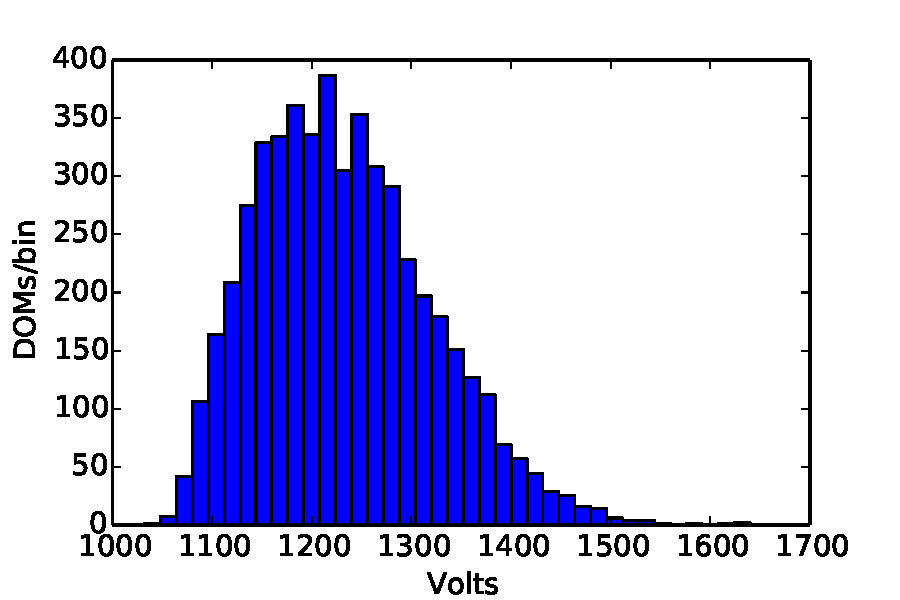
\includegraphics[width=0.6\textwidth]{graphics/dom/domcal/inice_hv_2016.pdf}
 \caption{PMT high voltage at $10^7$ gain for in-ice DOMs.}
 \label{fig:domcal_hv_settings}
\end{figure}

\subsubsection{\label{sec:domeff} DOM Optical Efficiency}

The UV photon detection efficiency in air is measured in the lab using a
pulsed 337~nm laser beam through a nitrogen gas chamber~\cite{ICECUBE:PMT}. Photons
which are Rayleigh scattered 90$^{\circ}$ from the beam illuminate the PMT,
which is rotated at various angles to measure different sections of
the photocathode surface. The quantum efficiency at the center of the
photocathode, where collection efficiency is nearly 100\%, was found
to be 20\% at 337~nm, which agrees well with the Hamamatsu
specification of 25\% at 390~nm. Lab measurements of the absolute efficiency of the DOM efficiency in water are ongoing~\cite{ICECUBE:DOMEFF}. The absolute calibration was performed on a small subset of IceCube DOMs. The relative efficiency of all DOMs was measured in the FAT process using a 405~nm pulsed laser and a system of fibers and diffusers to illuminate the DOM evenly within 50$^{\circ}$ of the optical axis; the DOM was not rotated for this measurement. The efficiency of each DOM was measured relative to a 2~inch reference PMT. The PMTs in most DeepCore DOMs are high quantum efficiency, nominally 40\% higher than PMTs in standard IceCube DOMs. FAT measurements found that the high quantum efficiency PMTs were 39\% more efficient than standard IceCube PMTs~\cite{ICECUBE:DC}.

Laboratory measurements of PMT efficiency are supplemented with in situ measurements using Cherenkov light from muons in the ice. Low energy muons (median energy 82~GeV) with inclination angles between 45$^{\circ}$ and 70$^{\circ}$ have well understood light emission and illuminate the downward-facing PMTs in the ice as directly as possible. The deposited charge from these muons is compared to simulation to adjust the effective efficiency of the PMTs in ice~\cite{IC3:ereco}. DOM occupancy from muons was used to measure the relative efficiency of the HQE and standard DOMs in ice, which was found to be 35\%~\cite{ICECUBE:DC}. The dark noise rates in HQE DOMs are 33\% higher than in standard DOMs.


%\subsubsection{Flasher Calibrations}

\subsection{Performance and Reliability}

As the DOMs are not serviceable after deployment, an extensive testing
protocol including temperature-cycling and cold-soaking ensured that bad
modules and early component failures were identified before shipping.
All DOMs were also re-tested at the South Pole before final deployment, to
screen out any modules damaged during transit.

As of 2016, 5397 of the 5484 deployed DOMs ($98.4\%$) are operating in
data-taking mode in the data acquisition system (see Table
\ref{tab:dom_failures}).  We classify DOM 
failures into two broad categories: failures during deployment and
freeze-in, and failures during subsequent operation.  The majority of the
failures (55) occurred before post-deployment commissioning; we hypothesize
that these are primarily attributable to cable failures, water leaks,
or freeze-in damage. 32 DOMs have failed after commissioning, and
we include in this count modules on a wire pair taken out of service when
the partner DOM on the same pair failed.  No particular pattern in the
failures is observed, other than they are typically during non-standard
operation or an exceptional event: a power outage, calibration run, or
flash filesystem upgrade.  The most recent two DOMs failed on May 23, 2013,
losing communications after a power outage.  Diagnosis of DOM failures
beyond identifying electrical shorts is challenging.

A number of DOMs have developed issues that affect their data-taking
configuration but are still usable.  The local coincidence settings of DOMs of
functional DOMs adjacent on a string to dead DOMs must also be
modified. These are enumerated in Table \ref{tab:dom_failures}.  

\begin{table}[h]
  \centering
  \begin{tabular}{| r | c |}
    \hline
    \bf{DOM failures} & \bf{87} \\
    \hline    
    deployment / freeze-in & 55 \\
    post-commissioning & 32 \\
    \hline
    \hline
    \bf{DOMs in Non-standard Mode} & \bf{171} \\
    \hline
    bad digitizer & 12 \\
    reduced PMT gain & 1 \\
    non-standard local coincidence & 158 \\
    \hline    
  \end{tabular}
  \caption{Number of DOM failures during deployment/freeze-in and after
    commissioning during detector operation, as well as DOMs with various
    issues (including a failed neighbor) causing them to be operated in a
    non-standard data-taking mode.} 
  \label{tab:dom_failures}
\end{table}

We can estimate the surviving fraction of DOMs 25 years after the original
deployment, assuming a constant, random failure rate after freeze-in.
Specifically, we calculate the Wilson score binomial confidence interval of
survival probability using the post-commissioning failure rate of DOMs
\cite{Wilson_Score}.  The estimated survival fraction as a function of
time is shown in Fig.~\ref{fig:dom_survival}; currently we estimate the
surviving fractEion in 2030 to be $97.3\pm0.3\%$.  While this simplified
model does not account for an increase in failure rate due to component aging, the
observed failure rate since detector completion of $2.0~\mathrm{yr}^{-1}$ is
significantly lower than the mean predicted rate of $4.5~\mathrm{yr}^{-1}$.  We attribute
this to infant mortality and/or to improved operational protocols that
minimize the number of DOM power cycles.

\begin{figure}[!h]
 \centering
 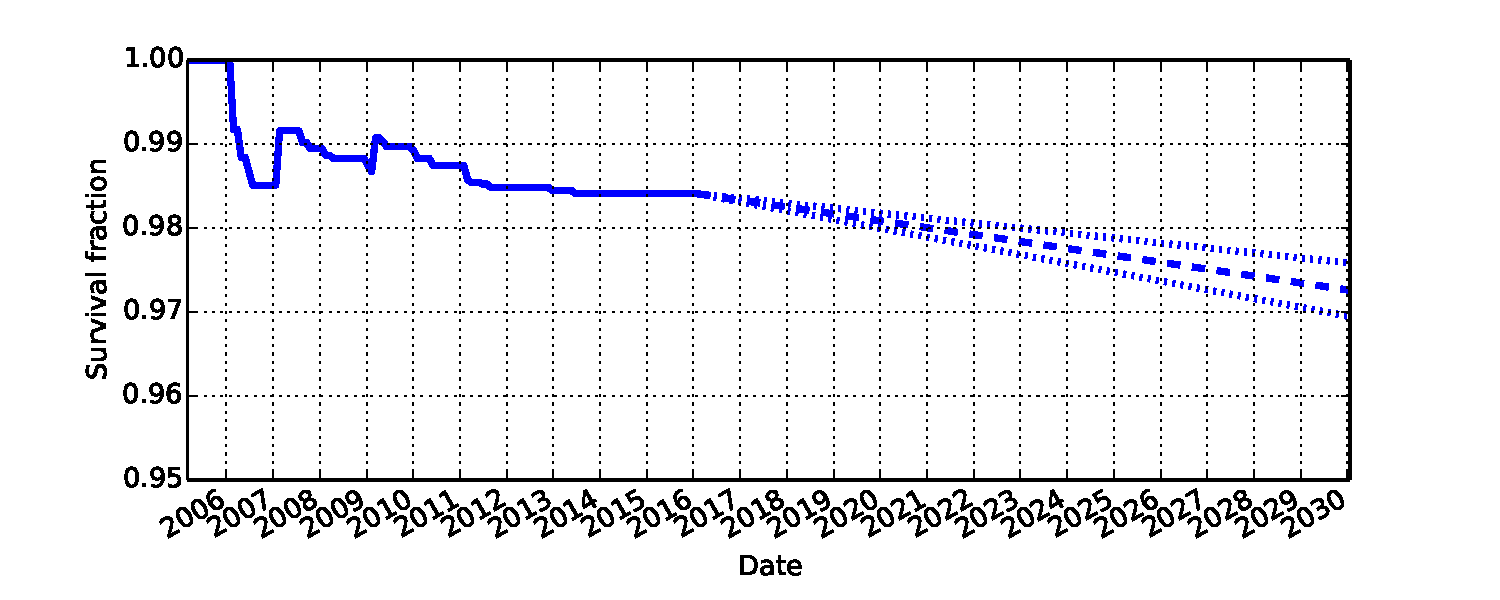
\includegraphics[width=0.95\textwidth]{graphics/dom/reliability/dom_survival.pdf}
 \caption{Actual and predicted fraction of surviving DOMs versus time, based on an assumed
 constant post-freeze-in failure rate.  The dotted lines indicate the
 central and 95\% CL estimates.  Increases before 2011 are due
 to deployments of new strings.} 
 \label{fig:dom_survival}
\end{figure}

%We have over $N$ DOM years in ice.  What can be said about 
%the reliability?  This section could be quite important.

\subsubsection{Baseline Stability}

An ATWD waveform consists of readouts from 128 independent digitizers,
while an FADC waveform consists of successive outputs of a 6-stage
pipelined digitizer (3 bins for SLC launches and 256 for HLC
launches). Two calibration constants are needed to turn each of these
raw digitizer readout values (an integer number of ADC counts) into a
voltage, from which the deposited charge is calculated. The deposited
charge is the basis for all energy measurements in IceCube. The
calibration constants needed are 1) the pedestal, the value the digitizer reads when the input voltage is zero, and
2) the gain, the input voltage required to increase increase the readout value by one count. 

Since each bin of each ATWD channel is read from an independent
digitizer, it is important to distinguish between the pedestals of
individual bins and the common pedestal of the entire waveform. The
baseline is the mean of the pedestals of each bin in a waveform. For
the FADC, this is the same as the pedestal. The pedestal pattern is
the deviation of each bin's pedestal from the common baseline. For the
FADC, this is identically zero. Since 2008, the DOM has subtracted the
pedestal pattern from
the ATWD waveform before sending it to the surface. The pedestal pattern is computed at the beginning of each
run by comparing 25 averaged pedestals. The autocorrelation coefficent
between the pairs of averaged pedestals is computed to detect light
contamination in the pedestals, and the shift between the baseline of
the pairs is calculated to determine that the baseline is stable. This
procedure ensures that fewer than 1 DOM in 1000 runs will contain a
contaminated baseline. Thereafter, both ATWD
and FADC waveforms can be calibrated by first subtracting the common
baseline from each bin, then multiplying by the gain. Correct
measurement of the common baseline is critical to correct charge
measurement and energy reconstruction.

The baseline is set to about 10\% of the maximum value of the
digitizer counts in
order to capture signals that go below the baseline. Since 2012, the baseline value is set by the DAQ configuration in order to ensure
stability. The baseline value differs for each digitizer channel in
each DOM, ranging from 112 to 161 counts in the fACD and 109 to 172
counts in the ATWD. The baselines for each digitizer channel in each DOM are monitored with
beacon hits, forced triggers which are collected at a rate of 1.2~Hz
per DOM
in in-ice DOMs and 4.8~Hz in IceTop DOMs. The average value of the
beacon baselines are very stable, with shifts of no more than
0.2~counts year to year, which corresponds to a stability of 0.05~PE
in the single photoelectron charge peak. 
%igures go here: average beacon waveform, stability, sample values
%for beacon baselines
The baselines are sensitive to radio frequency interference (RFI). In
2009, RF signals from a radar transmitter broadcasting at 46.3~MHz
appeared as sinusoidal or spiky signatures in the waveform
baselines. Also in 2009, a DOM 68-42 ``Krabba'' was damaged by a too-high
voltage setting during DOM calibration, and appeared to begin
sparking, causing sinusoidal waveforms to appear in the baselines of
neighboring DOMs.
%more figures go here: waveforms from Krabba disaster and Meteor radar

\subsubsection{Gain Stability}

The gain stability of the DOM, or the stability of the amplified charge
from converted photons, depends on a number of factors including stability
of the PMT high voltage, Main Board channel amplifiers, and the digitizers.
We can examine these subsystems using both historical calibration results
as well as by tracking the SPE charge during data-taking.

The electronic gain stability of the DOM includes variations in the
front-end electronic amplifiers and the digitizers themselves.  The
stability is checked by comparing the Main Board channel amplifier gains
from sets of calibrations taken from 2011 to 2016 (see
Fig.~\ref{fig:domcal_ch_gain}).  From year to year, the amplifier gain
calibration is repeatable to 0.1\%, 0.2\%, and 0.5\% in the high-gain,
medium-gain, and low-gain channels respectively.  Since detector completion
in 2011, a small systematic shift of $-0.3\%$ is visible in the low-gain
channel, but this is corrected by updating the calibration constants of
each DOM.

% JK: DOMCal History.ipynb
\begin{figure}[!h]
  \captionsetup[subfigure]{labelformat=empty}
  \centering
  \subfloat[]{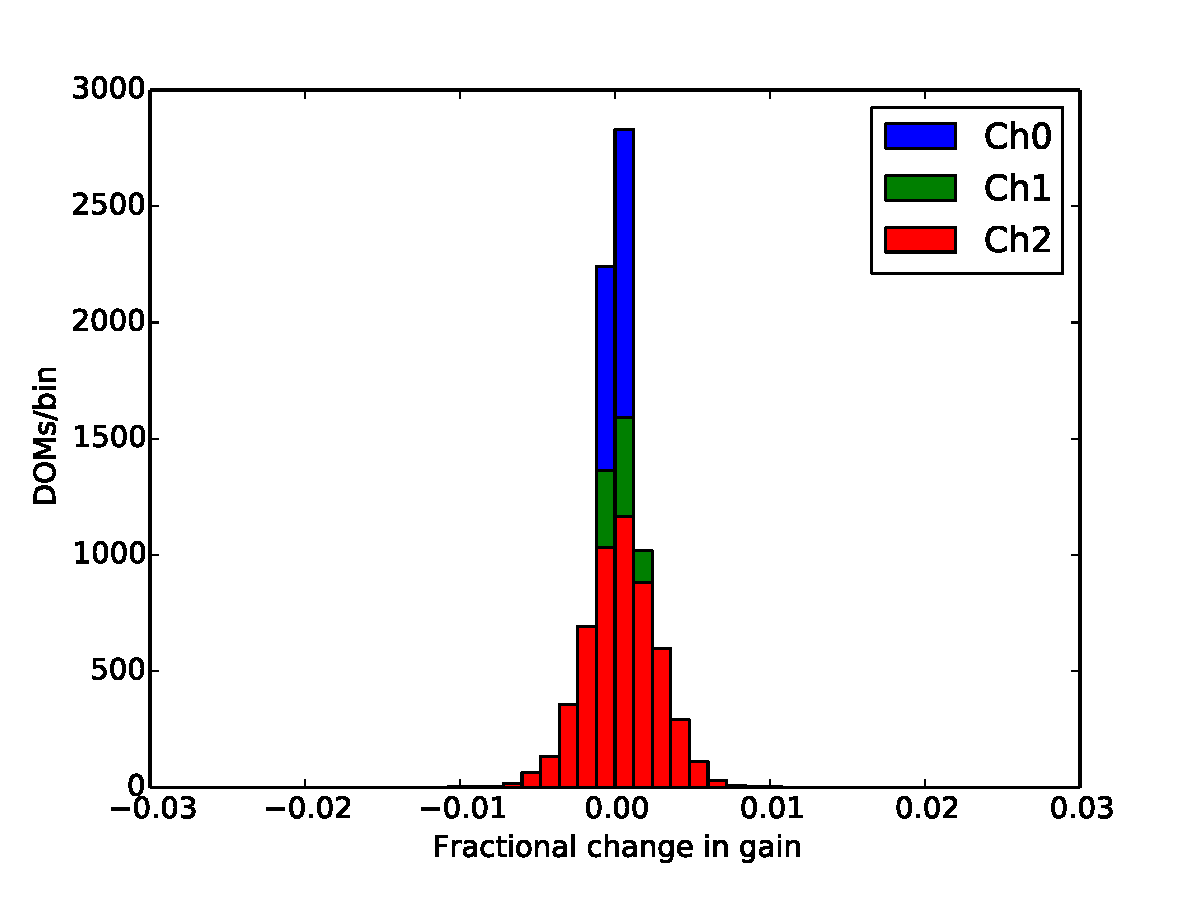
\includegraphics[width=0.5\textwidth]{graphics/dom/reliability/channel_gain_shift_2016_2015.pdf}}
  \subfloat[]{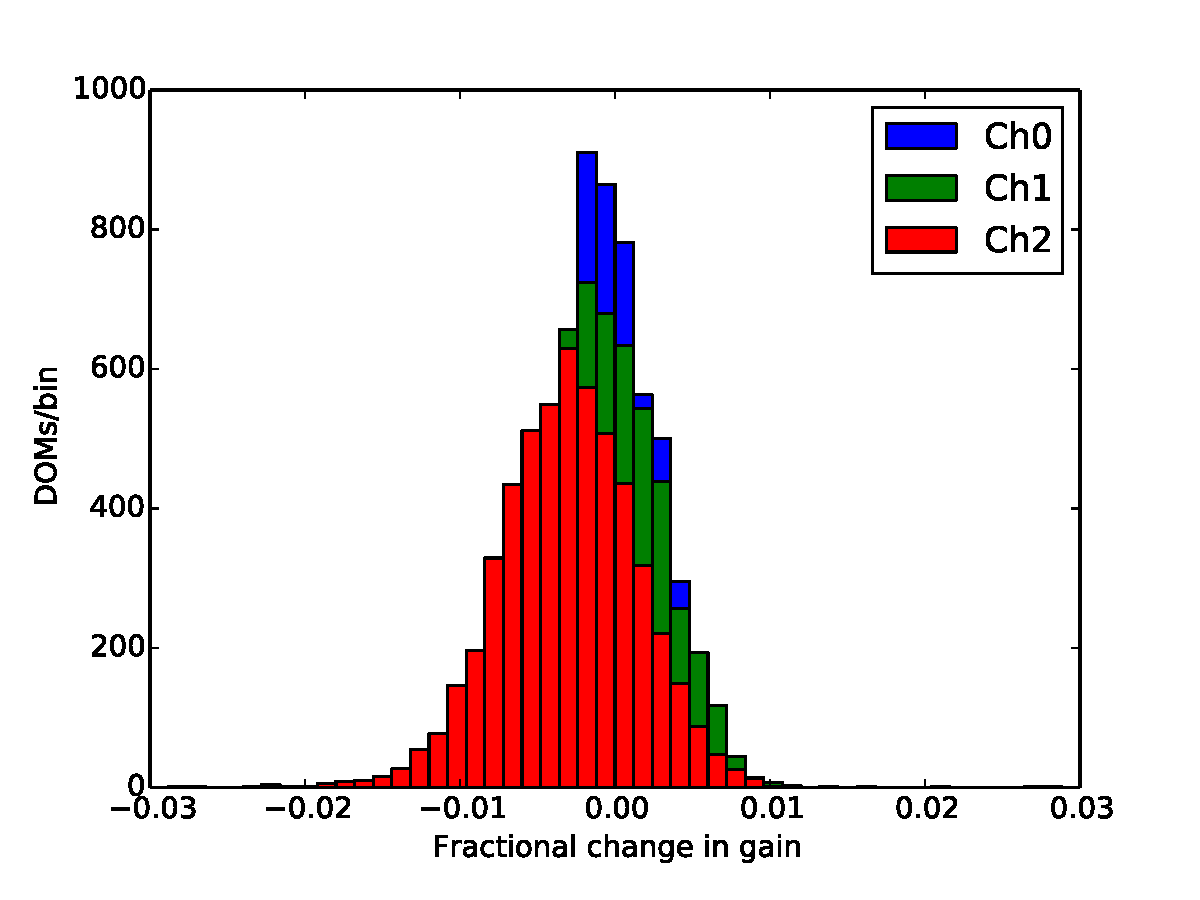
\includegraphics[width=0.5\textwidth]{graphics/dom/reliability/channel_gain_shift_2016_2011.pdf}}
  \caption{Fractional DOM channel amplifier gain shifts, from 2015 to
    2016 (left) and 2011 to 2016 (right).  Channels 0, 1, and 2 are
    high-gain, medium-gain, and low-gain respectively.}
  \label{fig:domcal_ch_gain}
\end{figure}

The PMT gain stability is monitored during data-taking using the
single photoelectron peak of the charge distribution on each DOM. A
Gaussian is fit to the peak region and the mean of the Gaussian is
tracked throughout the year. The peak position is calibrated to 1~PE
and is stable to within 0.01~PE for 95\% of all DOMs. There are on the
order of 12~DOMs which show unpredictable, abrupt shifts in the SPE peak
position of 0.05~PE or more. Figure XX shows the time history of the
SPE peak position of one of these DOMs over XX months. The peak shift
corresponds to increases or decreases in the MPE discriminator rate,
indicating that the SPE peak shift is caused by a change in the DOM
gain. 

\subsubsection{Optical Sensitivity Stability}

The detector response in IceCube is calibrated with low energy muons as
described in \cite{IC3:ereco}. The detector response is monitored in each run using the track
detection probability (TDP) calculated from high
multiplicity muon tracks with more than 30 hits in IceCube. The muon
tracks are reconstructed using the likelihood methods described in
\cite{IC3:ereco}; charge and time information from the DOM under study excluded
from the reconstruction. The TDP is
defined for each DOM as the ratio of the number of detected tracks
within 100~m of the DOM to the total number of tracks within 100~m of
the DOM. This ratio depends both on the optical properties of the ice
near the DOM and the optical efficiency of the DOM. We do not attempt
to separate
these effects in the TDP, but rather use the TDP to monitor the
overall stability of the detector response. Figure XX shows the TDP on
string 80, which includes both standard and HQE DOMs; the TDP is
20\% - 25\% higher for HQE DOMs than for neighboring standard
DOMs. The TDP is stable to within 1\% since 2012, when the baselines
were stabilized by being set in the DAQ configuration. Figure XX shows
the difference in the TDP for all DOMs between a run in 2012 and a run
in 2015.
%Figure goes here: TDP on string 80, showing the jump in DOMs 30-43
%which are HQE
%Figure goes here: TDP difference between 2012 run (after April 29)
%and 2015 run.

The detector response stability is also measured with the {\it in
  situ} light sources in IceCube. Both the in-ice calibration laser
\cite{IC3:SC} and the flasher LEDs show less than 1\% difference in the total
charge collected between 2012 and 2015. 

\subsubsection{Dark Noise}


The vast majority of background hits result from dark noise, i.e. effects that lead to the emission of an electron from the cathode of the PMT in the absence of an external photon. The total hit rate of DOMs with normal quantum efficiency PMTs is on average \SI{560}{\hertz} and \SI{780}{\hertz} for high QE DOMs. 
The dark noise is composed of two major components. Electronics noise and radioactive decay in the material form the uncorrelated noise pulses of Poissonian nature with a rate between \SI{230}{\hertz} and \SI{250}{\hertz} that follows the Richardson law for thermal emission. 
The remaining component is the so-called correlated noise
with a hit rate that increases with decreasing temperature from \SI{280}{\hertz} to \SI{340}{\hertz} (Figure \ref{fig:dom_darknoise_vs_temperature}). 
This temperature dependent noise rate profile was acomplished by combining a measured temperture profile of the the South Pole ice cap \cite{price2002temperature} with a fit of the Poissonian expectation to the total dark noise rate to every individual DOM.

\begin{figure}
 \begin{minipage}[t]{0.45\linewidth}
 \centering
  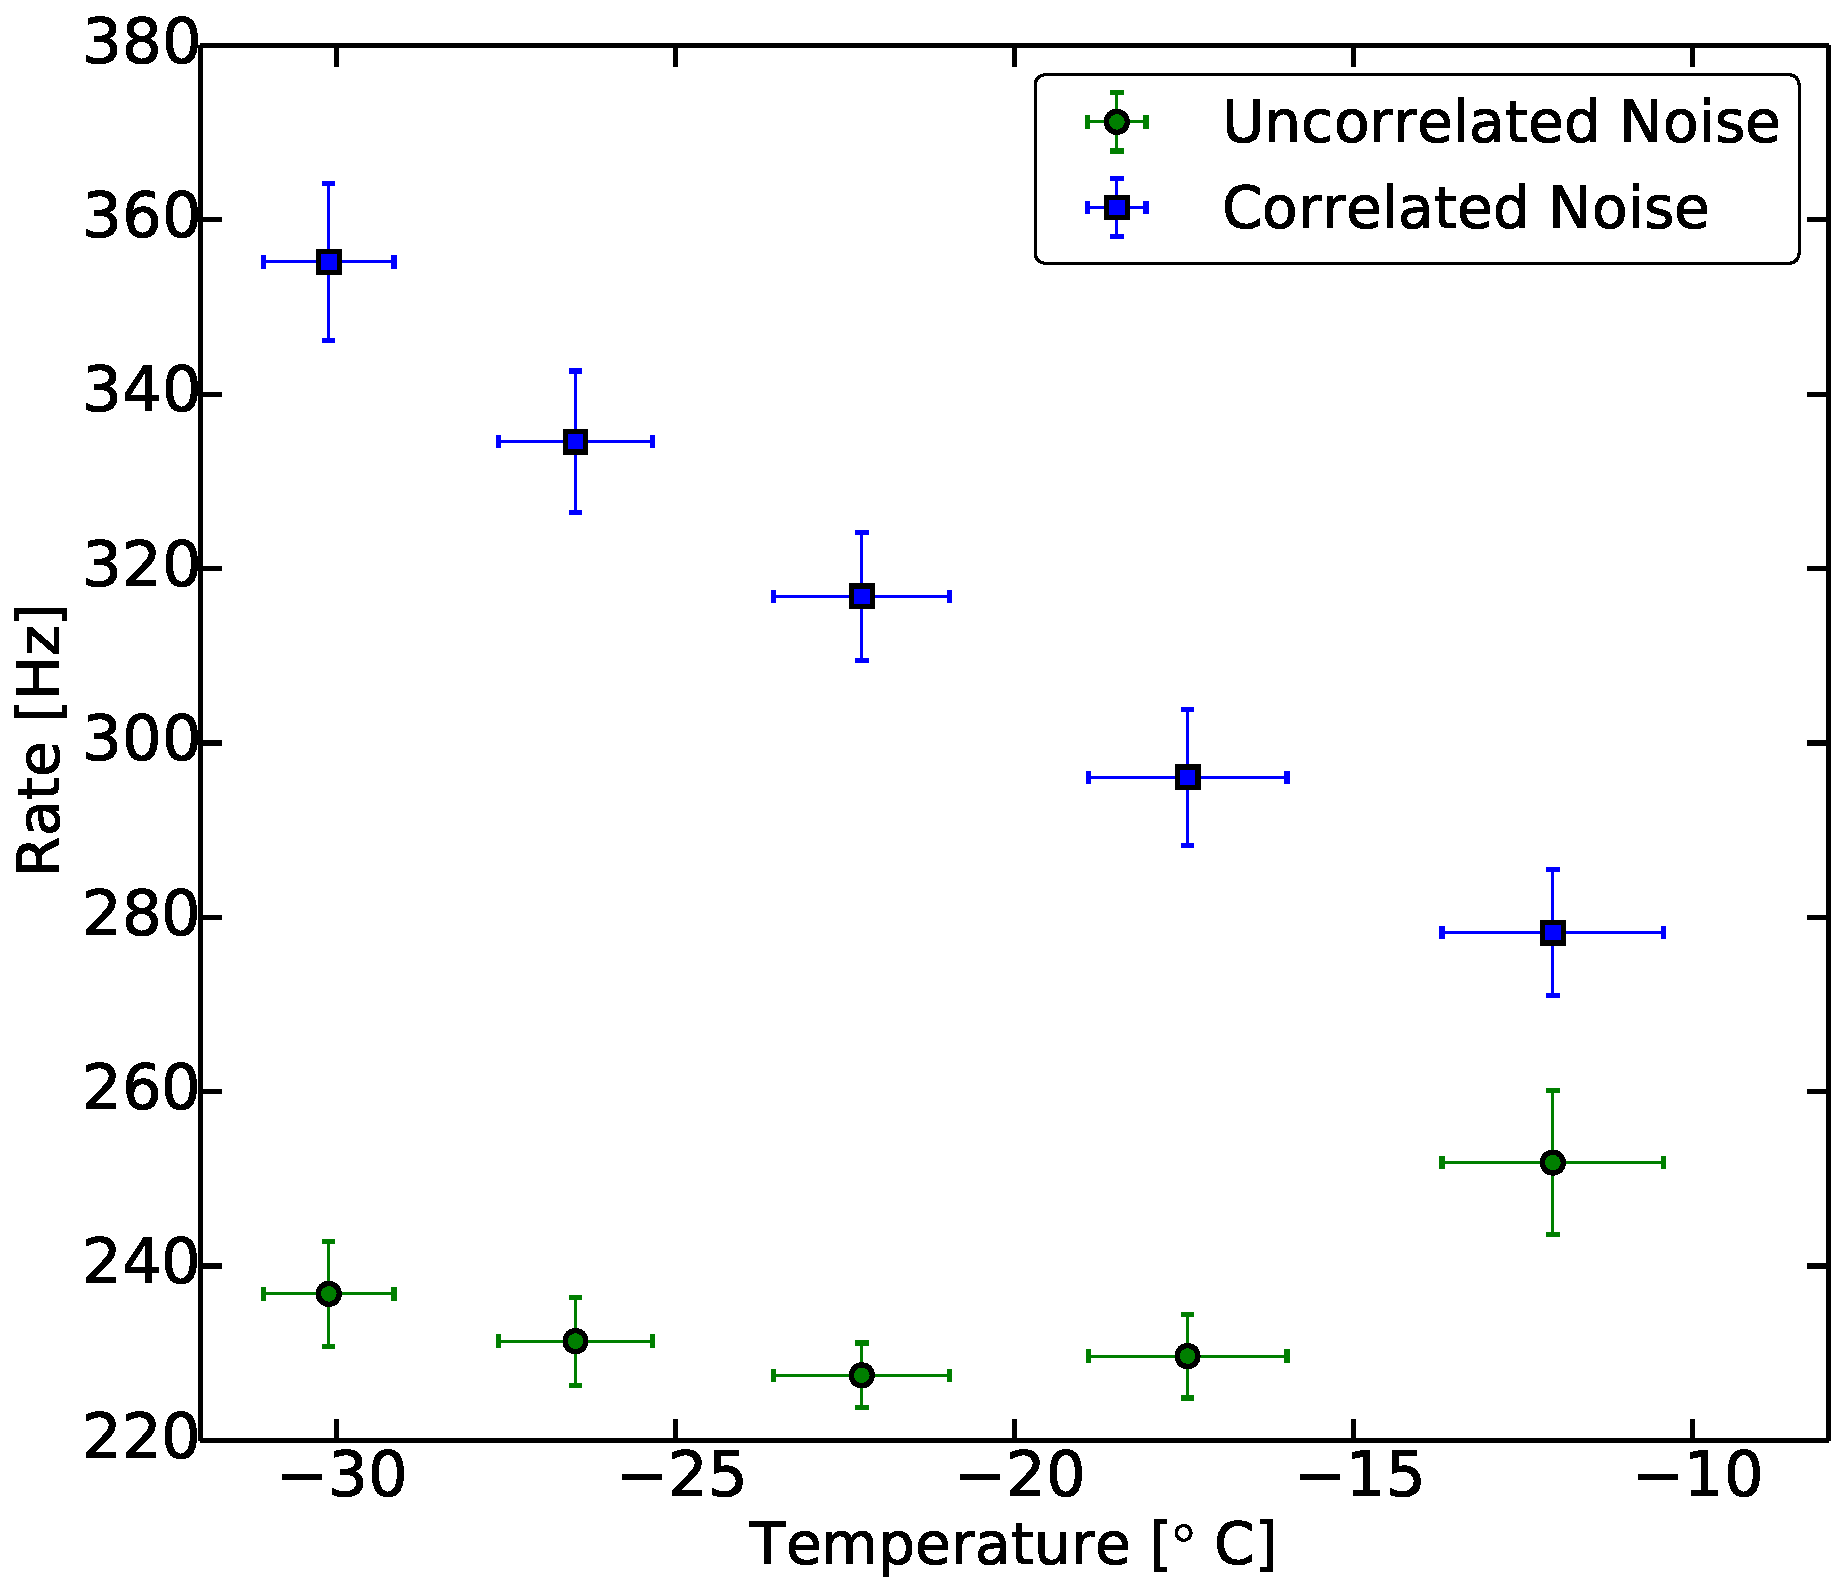
\includegraphics[width=\textwidth]{graphics/dom/performance/darknoise/HitRatevsTemp_inice_nomuons_nofit_bigfont.pdf}
 \caption{Dark noise rate in IceCube as a function of temperature, obtained from hitspooling
 data. Each data point represents the average of 12 DOM layers from 78 strings (DeepCore excluded)}
 \label{fig:dom_darknoise_vs_temperature}
 \end{minipage}
\hfill
 \begin{minipage}[t]{0.45\linewidth}
 \centering
  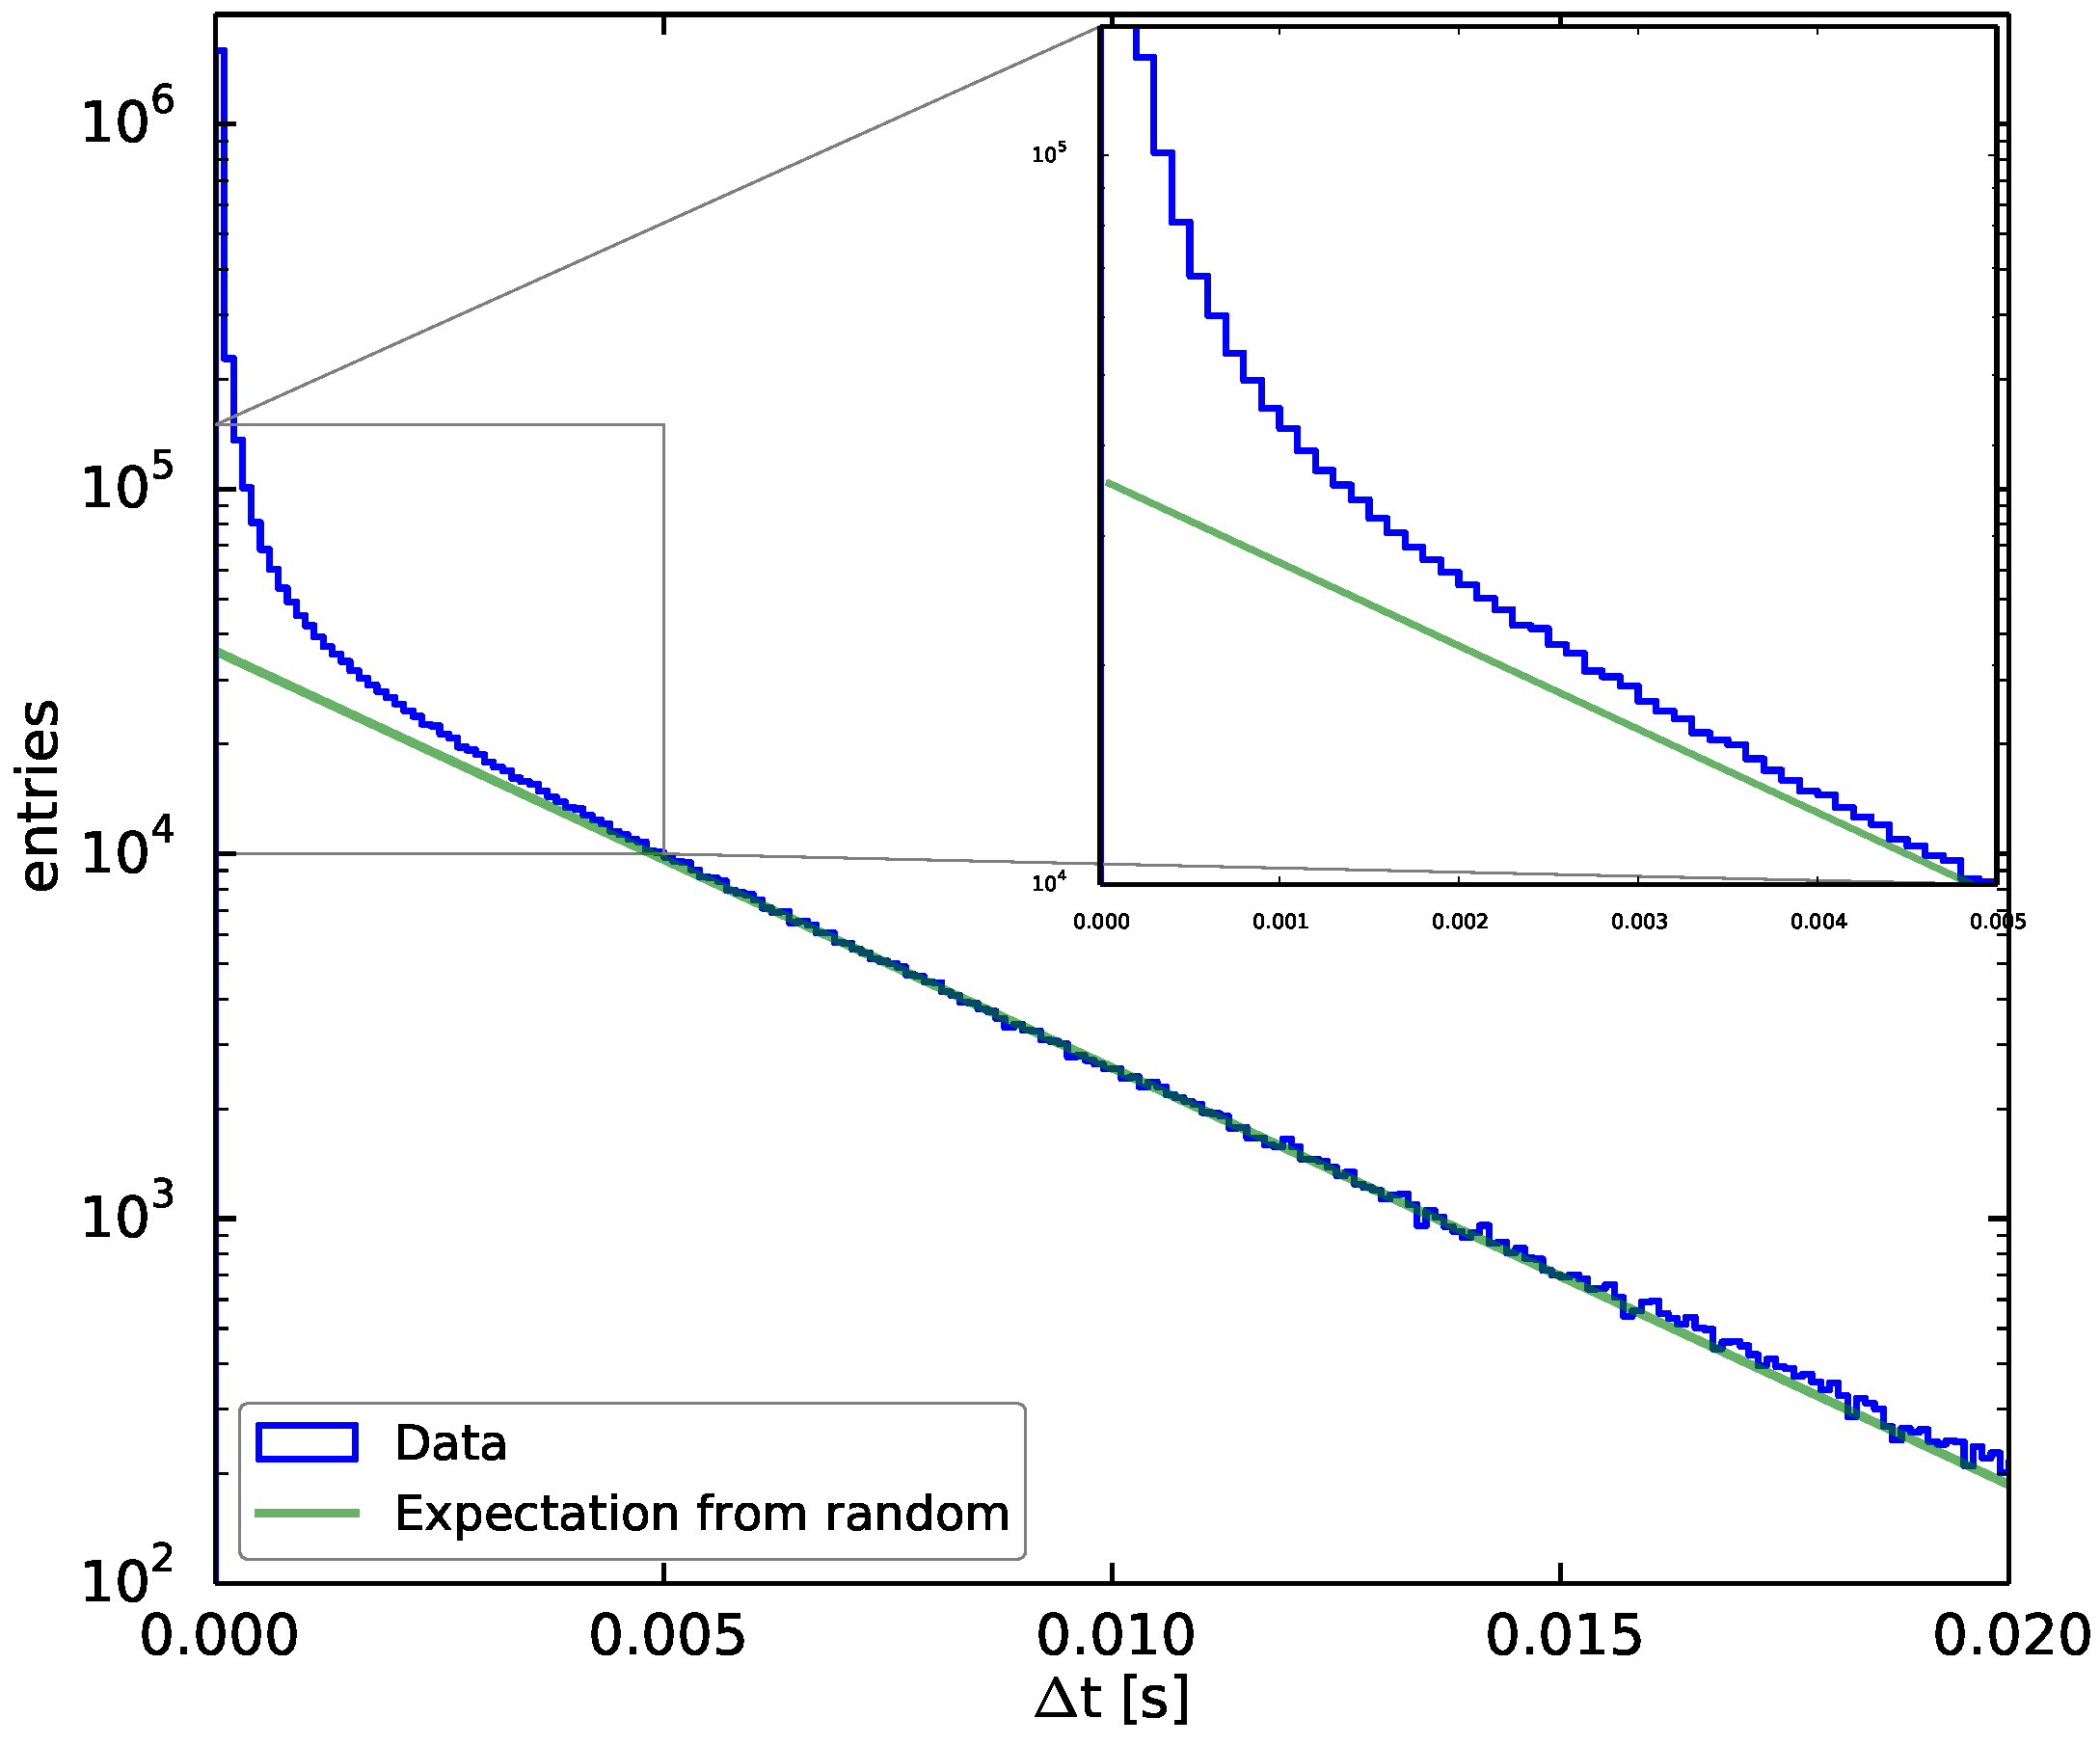
\includegraphics[width=\textwidth]{graphics/dom/performance/darknoise/DarkNoise_Layer2Doms.pdf}
 \caption{Time interval between successive hits for all next-to-top layer DOMs (DeepCore excluded).}
 \label{fig:darknoise_deltaT}
 \end{minipage}
\end{figure}

The correlated noise component manifests itself in an overabundance of short time intervals between hits in a single DOM compared to the expectation from random (Figure \ref{fig:darknoise_deltaT}). The short time intervals are correlated and clustered in bursts with an average number of hits per burst rising from \num{3.3} at \SI{-10}{\celsius} to \num{3.8} at \SI{-30}{\celsius}. A detailed study with hitspooling data shows that the phenomenology of the correlated noise component in Icecube is in general in good agreement with results reported in the literature with a satisfying physical explanation still to be determined. Best candidate for the source of the entire process is luminescence triggered by radioactive decay of elements like Thorium and Uranium in the glass of the DOM.
The various sources of dark noise are best visible when histogramming the time between susequent hits in a DOM on a logarithmic scale, as shown in Figure \ref{fig:darknoise_deltaT_components}. Several noise components could be identified and are summerized in Table \ref{tab:noise}.
Icecube uses the result of these studies to build a parametrized noise model that is needed for an acurate detector simulation \cite{larson2013simulation}.

\begin{table}[h!]
\caption{Characteristics of noise components in IceCube DOMs, adapted from \cite{stanisha_noise_14}.}
  \centering
  \footnotesize
\begin{tabularx}{\textwidth}{lXXX}
\toprule
Noise Component& Origin & Distribution & Parameters \\
\midrule
Afterpulses & PMT & Gaussian & $\mu = \SI{6}{\micro\second}$ \newline $\sigma = \SI{2}{\micro\second}$\\
Uncorrelated & Thermal noise\newline Radioactive Decay & Poissonian & $\lambda = \sim \SI{250}{\hertz}$\\
Correlated & Luminescence (?) & Log-normal & $\mu = \num{-6} [\log_{10}(\frac{\Delta T}{s})]$ \newline $\sigma = \num{0.85} [\log_{10}(\frac{\Delta T}{s})]$\\
\bottomrule
\end{tabularx}
\label{tab:noise}
\end{table}

\begin{figure}[!h]
 \centering
  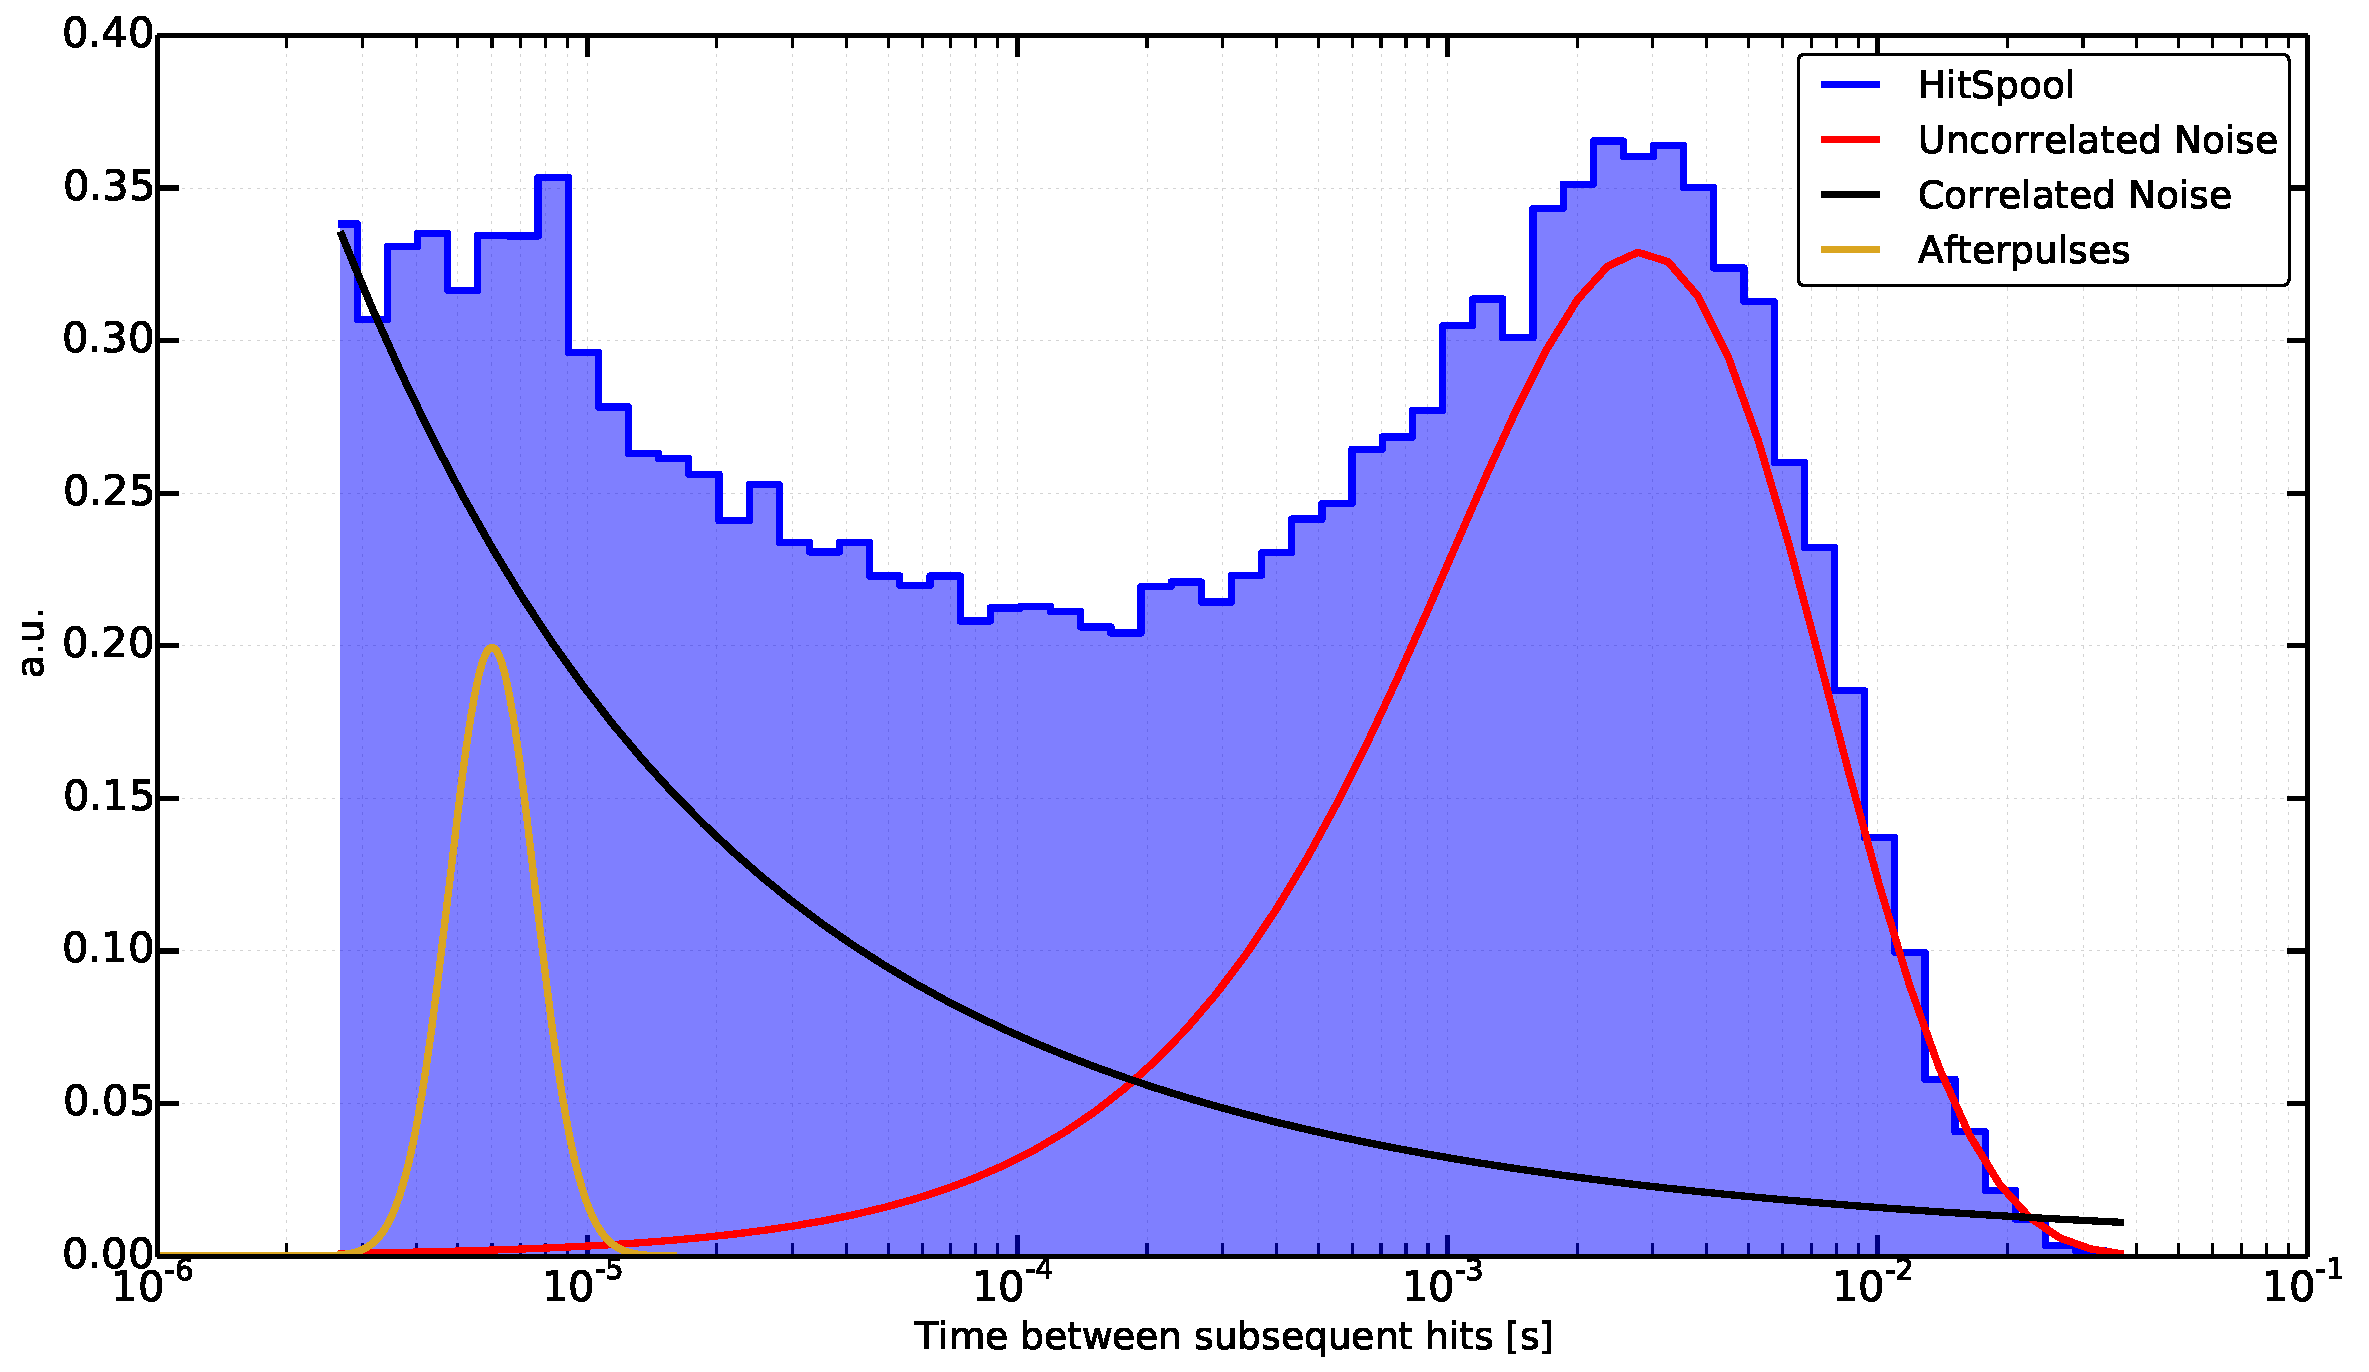
\includegraphics[width=0.8\textwidth]{graphics/dom/performance/darknoise/SingleDOM_HitSpool_Hits_deltaT_fits_example.pdf}
 \caption{Histogram of time differences between successive hits from HitSpool data of
DOM 15-27 (blue) on a logarithmic scale in order to visualize the different noise components
(without prepulses which are comparatively insignificant) \cite{heereman2015hitspooling}.}
 \label{fig:darknoise_deltaT_components}
\end{figure}


The dark noise evolution over time was investigated using data from the supernova scaler stream \cite{briedel_phd}. There is a exponential decay over the course of the data set. This is especially recognizable in the standard deviation of the distribution. The standard deviation decreases by 25\% over the
course of the three years, and is not noticeably effected by the seasonal modulation. Changes in the mean are initially
dominated by the decay component and later by the seasonal variation of the atmopsheric muons. 


\begin{figure}[!h]
 \centering
 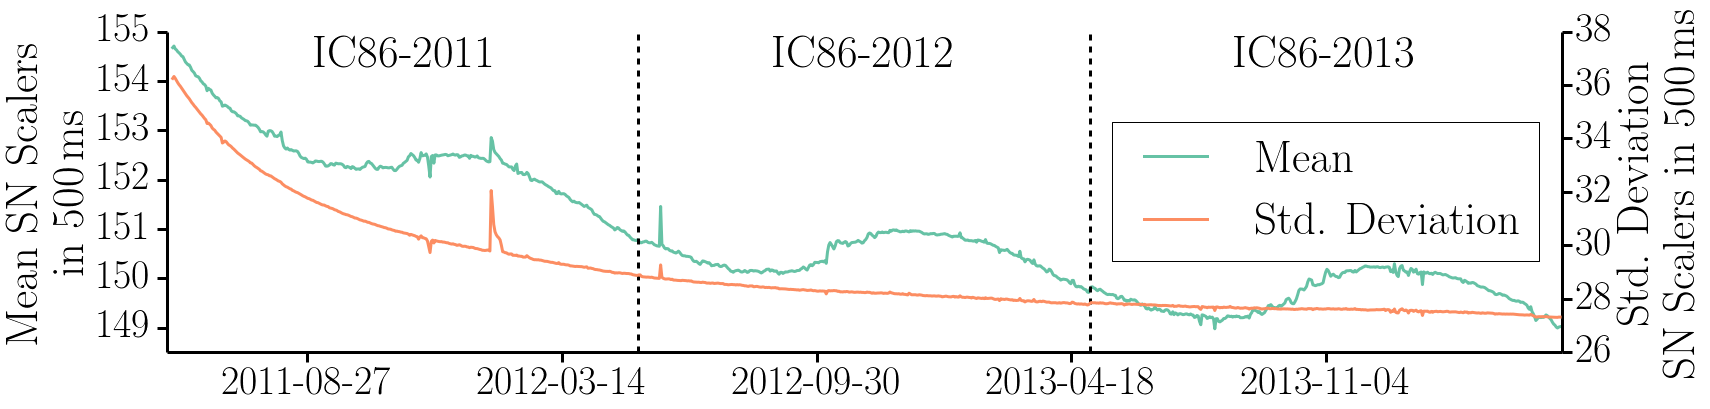
\includegraphics[width=0.95\textwidth]{graphics/dom/performance/darknoise/briedel1.png}
 \caption{Mean and variance of the supernova scaler distribution for the entire detector over the course of the first three
years of the completed IceCube \cite{briedel_phd}.}
 \label{fig:noise_over_time_briedel}
\end{figure}


\begin{figure}[!h]
 \centering
 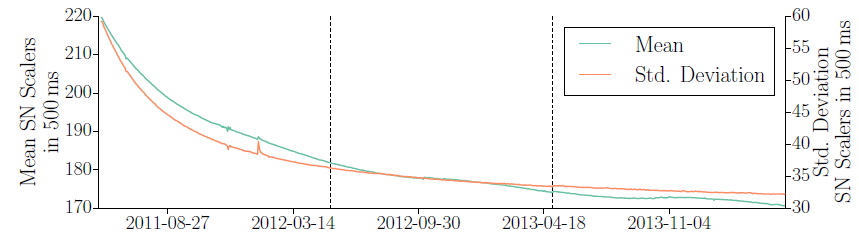
\includegraphics[width=0.95\textwidth]{graphics/dom/performance/darknoise/briedel4.png}
 \caption{Mean and standard deviation of the scaler rate of strings deployed in the last deployment season (austral summer of 2010/2011) \cite{briedel_phd}.}
 \label{fig:noise_over_time_briedel}
\end{figure}


\begin{figure}[!h]
 \centering
 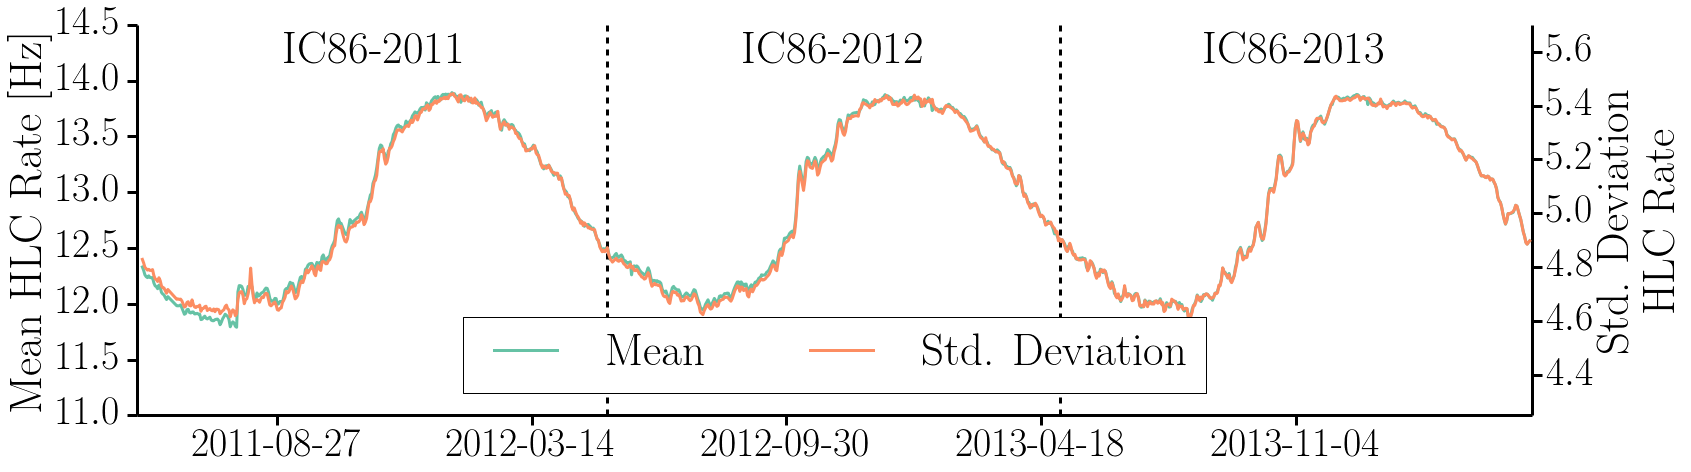
\includegraphics[width=0.95\textwidth]{graphics/dom/performance/darknoise/briedel2.png}
 \caption{Mean and standard deviation of the HLC rate distribution \cite{briedel_phd}.}
 \label{fig:slc_over_time_briedel}
\end{figure}

\begin{figure}[!h]
 \centering
 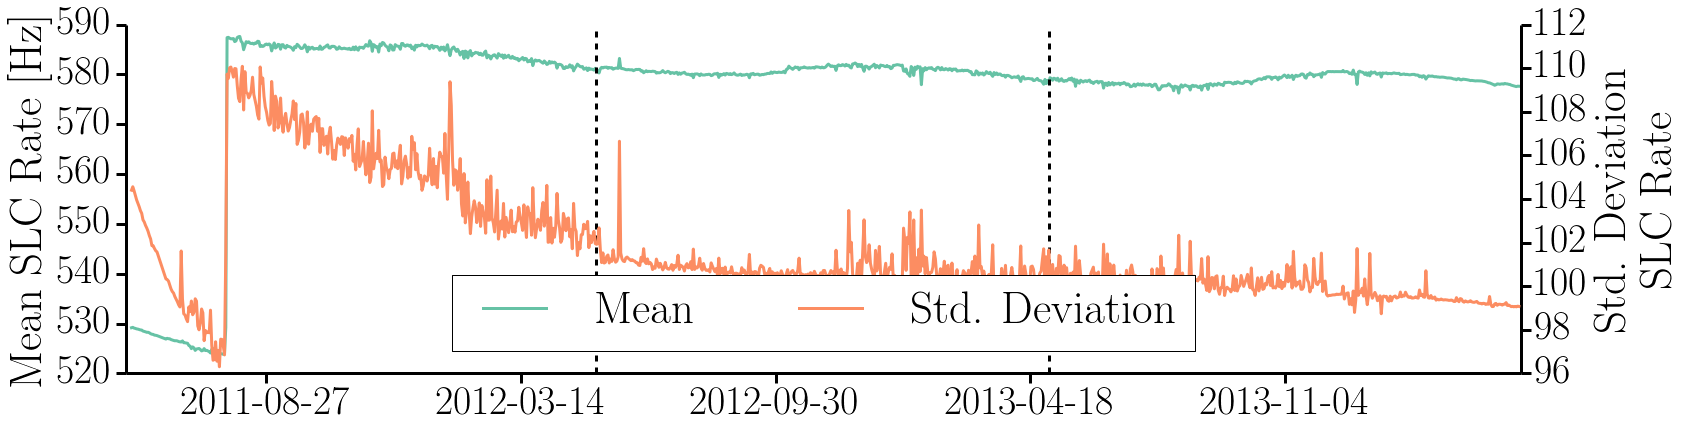
\includegraphics[width=0.95\textwidth]{graphics/dom/performance/darknoise/briedel3.png}
 \caption{Mean and standard deviation of the SLC rate distribution. The decay and jump in both quantities result from a change in the DOM deadtime by 10\%. \cite{briedel_phd}.}
 \label{fig:hlc_over_time_briedel}
\end{figure}










%%%%%%%%%%%%%%%%%%%%%%%%%%
%
% following refs should be moved to top level
%
%%%%%%%%%%%%%%%%%%%%%%%%%%

%\begin{thebibliography}{9}

%IceCube energy reconstruction paper
%\bibitem{IC3:ereco} IceCube energy reconstruction paper

%IceCube standard candle reference
%\bibitem{IC3:SC} IceCube standard candle reference: Kiryluk et al proceedings ICRC 2007

%IceCube science description
%\bibitem{IC3:sci} IceCube Collaboration: J.~Ahrens {\it et al.}, Astropart. Phys. {\bf 20} (2004) 507

%IceCube original performance paper
%\bibitem{IC3:perf} IceCube Collaboration: A.~Achterberg  {\it et al.}, Astroparticle Physics {\bf 26} (2006) 155

%IceCube DOM-DAQ paper
%\bibitem{ref:domdaq}IceCube Collaboration: R.~Abbasi {\it et al.}, Nucl. Instr. and Methods in Phys. Res. A {\bf 601} (2009) 294

%IceCube PMT paper
%\bibitem{ref:pmt}IceCube Collaboration: R.~Abbasi {\it et al.}, Nucl. Instr. and Methods in Phys. Res. A {\bf 618} (2010) 139

%Characterization of large-area photomultipliers under low magnetic fields: 
%Design and performance of the magnetic shielding for the Double Chooz neutrino experiment
%\bibitem{ref:calvo} E.~Calvo {\it et al.}, Nucl. Instr. and Methods in Phys. Res. A {\bf 621} (2010) 222
%\end{thebibliography}
